\documentclass{lab_sheet}
\usepackage[flushleft]{threeparttable}
\usepackage[hidelinks]{hyperref}

\newcommand{\setting}[2]{
    \begin{tabular}{C{3cm}C{5cm}C{5cm}}
        \toprule
          #1 & IP address & Subnet mask\\
          \midrule
          #2
          \bottomrule
       \end{tabular}
}

\newcommand{\parameter}[1]{
    \begin{tabular}{C{3cm}C{2cm}C{2cm}C{2cm}C{2cm}}
        \toprule
        Router & hostname & console password & enable password& vty password\\
        \midrule
          #1 
          \bottomrule
       \end{tabular}
}

\newcommand{\customcaption}[2]{
    \begin{mdframed}[backgroundcolor=bg,innerbottommargin=-2.5em]
        \lstinputlisting[label={lst:#1},captionpos=b,style=DOS,caption={#2}]{./Outputs/#1.txt}
          \end{mdframed}
}
\newcommand{\ping}[1]{
    \begin{tabular}{||C{3cm}||C{5cm}||C{5cm}||}
        \toprule
          Sending Host & Destination & Ping status\\
          \hline
          #1
          \bottomrule
       \end{tabular}
}

\newcommand{\activityapingpc}[2]{
    \cmdop{#1-a}{ping test from #2 to PC1}
    \cmdop{#1-b}{ping test from #2 to PC3}
    \cmdop{#1-c}{ping test from #2 to PC5}
    \cmdop{#1-r0}{ping test from #2 to Router 0: 0/0}
    \cmdop{#1-r1}{ping test from #2 to Router 0: 0/1}
    \cmdop{#1-r2}{ping test from #2 to Router 0: 0/2}
    \cmdop{#1-r3}{ping test from #2 to Router 1: 0/0}
    \cmdop{#1-r4}{ping test from #2 to Router 1: 0/1}
}

\newcommand{\activitybpingpc}[2]{
    \cmdop{#1-a}{ping test from #2 to PC0}
    \cmdop{#1-b}{ping test from #2 to PC1}
    \cmdop{#1-c}{ping test from #2 to PC2}
    \cmdop{#1-d}{ping test from #2 to PC3}
    \cmdop{#1-e}{ping test from #2 to Server 0}
    \cmdop{#1-f}{ping test from #2 to Server 1}
    \cmdop{#1-r0}{ping test from #2 to Router 0: 0/0}
    \cmdop{#1-r1}{ping test from #2 to Router 0: 0/1}
    \cmdop{#1-r2}{ping test from #2 to Router 1: 0/0}
    \cmdop{#1-r3}{ping test from #2 to Router 1: 0/1}
    \cmdop{#1-r4}{ping test from #2 to Router 1: 0/2}
    \cmdop{#1-r5}{ping test from #2 to Router 2: 0/0}
    \cmdop{#1-r6}{ping test from #2 to Router 2: 0/1}
    \cmdop{#1-r7}{ping test from #2 to Router 2: 0/2}
    \cmdop{#1-r8}{ping test from #2 to Router 3: 0/0}
    \cmdop{#1-r9}{ping test from #2 to Router 3: 0/1}
}


\newcommand{\activitybshowroute}[1]{
  \foreach \i in {0,1,2,3}
  {
    \cmdop{#1-\i}{show ip route on Router \i}
  }
}

\newcommand{\activitybpingrouter}[2]{
    \cmdop{#1-a}{ping test from Router #2 to PC0}
    \cmdop{#1-b}{ping test from Router #2 to PC1}
    \cmdop{#1-c}{ping test from Router #2 to PC2}
    \cmdop{#1-d}{ping test from Router #2 to PC3}
    \def\argI{0}%
    \def\argII{1}%
    \def\argIII{2}%
    \def\argIV{3}%
    \def\temp{#2}%
    \ifx\temp\argI
    \cmdop{#1-r2}{ping test from Router #2 to Router 1: 0/0}
    \cmdop{#1-r3}{ping test from Router #2 to Router 1: 0/1}
    \cmdop{#1-r4}{ping test from Router #2 to Router 1: 0/2}
    \cmdop{#1-r5}{ping test from Router #2 to Router 2: 0/0}
    \cmdop{#1-r6}{ping test from Router #2 to Router 2: 0/1}
    \cmdop{#1-r7}{ping test from Router #2 to Router 2: 0/2}
    \cmdop{#1-r8}{ping test from Router #2 to Router 3: 0/0}
    \cmdop{#1-r9}{ping test from Router #2 to Router 3: 0/1}
    \fi
    \ifx\temp\argII
    \cmdop{#1-r0}{ping test from Router #2 to Router 0: 0/0}
    \cmdop{#1-r1}{ping test from Router #2 to Router 0: 0/1}
    \cmdop{#1-r5}{ping test from Router #2 to Router 2: 0/0}
    \cmdop{#1-r6}{ping test from Router #2 to Router 2: 0/1}
    \cmdop{#1-r7}{ping test from Router #2 to Router 2: 0/2}
    \cmdop{#1-r8}{ping test from Router #2 to Router 3: 0/0}
    \cmdop{#1-r9}{ping test from Router #2 to Router 3: 0/1}
    \fi
    \ifx\temp\argIII
    \cmdop{#1-r0}{ping test from Router #2 to Router 0: 0/0}
    \cmdop{#1-r1}{ping test from Router #2 to Router 0: 0/1}
    \cmdop{#1-r2}{ping test from Router #2 to Router 1: 0/0}
    \cmdop{#1-r3}{ping test from Router #2 to Router 1: 0/1}
    \cmdop{#1-r4}{ping test from Router #2 to Router 1: 0/2}
    \cmdop{#1-r8}{ping test from Router #2 to Router 3: 0/0}
    \cmdop{#1-r9}{ping test from Router #2 to Router 3: 0/1}
    \fi
    \ifx\temp\argIV
    \cmdop{#1-r0}{ping test from Router #2 to Router 0: 0/0}
    \cmdop{#1-r1}{ping test from Router #2 to Router 0: 0/1}
    \cmdop{#1-r2}{ping test from Router #2 to Router 1: 0/0}
    \cmdop{#1-r3}{ping test from Router #2 to Router 1: 0/1}
    \cmdop{#1-r4}{ping test from Router #2 to Router 1: 0/2}
    \cmdop{#1-r5}{ping test from Router #2 to Router 2: 0/0}
    \cmdop{#1-r6}{ping test from Router #2 to Router 2: 0/1}
    \cmdop{#1-r7}{ping test from Router #2 to Router 2: 0/2}
    \fi
}

\begin{document}
    \titlePage{Default Route and its Configurations}{November 26, 2020}
    \pagenumbering{gobble}
    \tableofcontents
    \pagebreak
    \listoffigures
    \pagebreak
    \listoftables
    \pagebreak
    \lstlistoflistings
    \pagebreak
    \pagenumbering{arabic}
    \section{Objectives}
    \begin{itemize}
        \item Familiarization with default route and its configuration.
    \end{itemize}
    \section{Required Tools}
    \subsection{Cisco Packet Tracer}
    Cisco Packet Tracer is a visual simulation software developed and distributed by Cisco Systems. Packet Tracer is a cross platform tool that allows simulated environment for modern computer network and network topologies.
    \section{Simulation Activities}
    \begin{figure}[H]
        \centering
        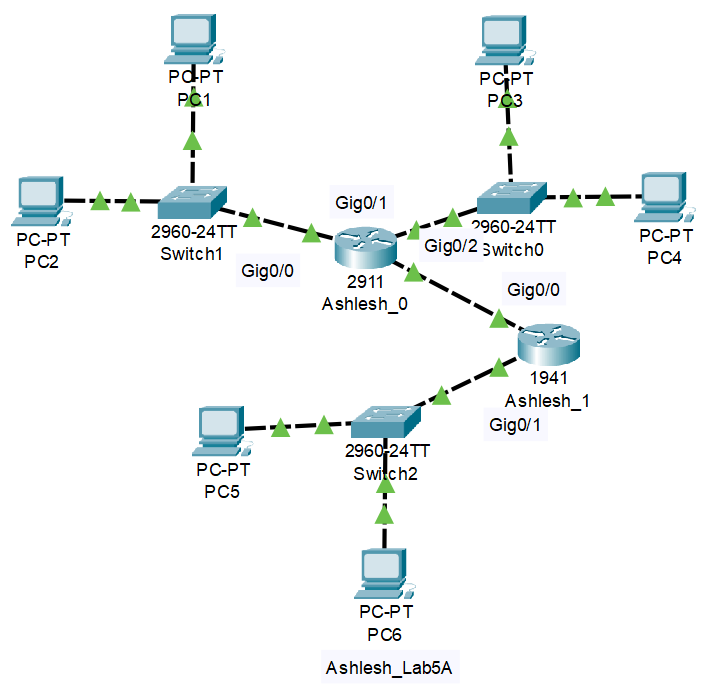
\includegraphics[scale=.8]{Figures/activitya.png}
        \caption{Simulated network for Activity A}
        \label{fig:activitya}
    \end{figure}

    \begin{figure}[H]
      \centering
      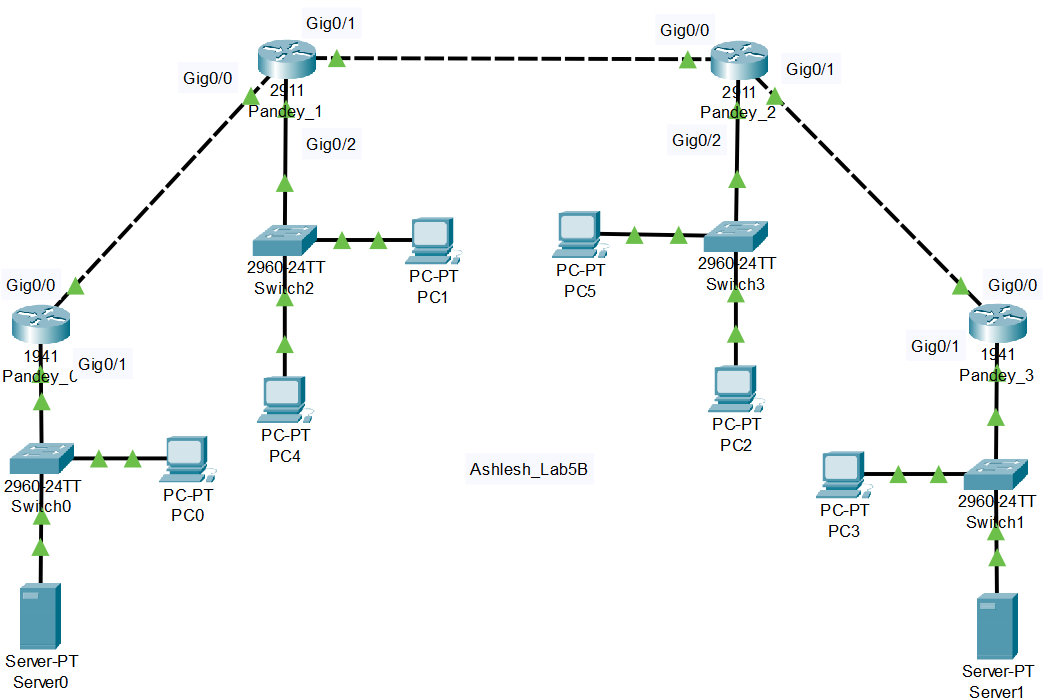
\includegraphics[scale=.6]{Figures/activityb.png}
      \caption{Simulated network for Activity B and C}
      \label{fig:activityb}
  \end{figure}


    \section{Exercises}
    \problem{What is a default route? Explain its significance.}
    Default route is a special kind of static route that is defined as the route the packets take when a router can't locate the destination host within its routing table. Static routes are defined as pre-set routes for packets corresponding to certain network identifiers, but this process of assigning routes can become hectic if there are multiple destination hosts that eventually need the same router as the next hop coming from the host. This is solved by defining a static route such that the packets that don't correspond to any entries in the routing table are forwarded to the immediate router with most number of connection, hence making it the default route for packets. Real life sitaution where default routes are used can be found in ISPs where the packets that don't have the destination address in the routing table are forwarded to an upstream ISP.\\
    The major significances of default route are:
    \begin{itemize}
      \item Reduction of entries in routing table.
      \item Reduction of latency within the router since unidentified packets are fowarded via the default route.
    \end{itemize}
    \problem{Explain the default route configuration command of router with its syntax.}
    \lstinputlisting[label={lst:syntaxrouting},caption={Syntax for configuring default route}, captionpos=b]{./Outputs/syntax.txt}
    \problem{Note down the observations of each step with necessary commands specified in activities
    A, B and C mentioned above and comment on it.}
    \subproblem{Activity A}

    \addtocontents{lol}{\protect\subsection*{Activity A}}
    \addtocontents{lot}{\protect\subsection*{Activity A}}
    \subsubsection*{Sub activity 1}
    \addtocontents{lol}{\protect\subsubsection*{Sub activity 1}}
    \addtocontents{lot}{\protect\subsubsection*{Sub activity 1}}
    The network shown in Figure~\ref{fig:activitya} is created using Packet Tracer with basic settings as,
    \begin{table}[H]
        \centering
        \begin{threeparttable}
        \setting{PC}{
        1 & 200.20.20.2  & 255.255.255.0 \\
        2 & 200.20.20.3  & 255.255.255.0 \\
        3 & 200.20.21.2  & 255.255.255.0 \\
        4 & 200.20.21.3  & 255.255.255.0 \\
        5 & 200.20.23.2  & 255.255.255.0 \\
        6 & 200.20.23.3  & 255.255.255.0 \\
        }
  \begin{tablenotes}
    \small
    \item Note: The ip addressess and subnet masks are set using the IP configuration application. The default gateways for the PCs were also set as, PC1 and PC2: 200.20.20.1, PC3 and PC4: 200.20.21.1, PC5 and PC6: 200.20.23.1
  \end{tablenotes}
  \caption{IP address and subnet masks for the PCs in the network}
  \label{tbl:pcsettinga}
        \end{threeparttable}
    \end{table}
    The gigabitethernet interfaces on the routers were set as,
    \begin{table}[H]
        \centering
        \begin{threeparttable}
        \setting{Gigabitethernet interfaces}{
        Router 0: 0/0 & 200.20.20.1  & 255.255.255.0 \\
        Router 0: 0/1 & 200.20.21.1  & 255.255.255.0 \\
        Router 0: 0/2 & 200.20.22.1  & 255.255.255.0 \\
        Router 1: 0/0 & 200.20.22.2  & 255.255.255.0 \\
        Router 1: 0/1 & 200.20.23.1  & 255.255.255.0 \\
        }
        \begin{tablenotes}
            \small
            \item Note: The ip addressess and subnet masks are set using the commands enlisted in Listings~\ref{lst:gigaset0} and \ref{lst:gigaset1}
          \end{tablenotes}
        \caption{IP address and subnet masks for the gigabitethernet interfaces on the routers}
        \label{tbl:gigasettinga}
    \end{threeparttable}
          \end{table}
          
          \customcaption{gigaset0}{Syntax for configuring interfaces on Router 0}
          \customcaption{gigaset1}{Syntax for configuring interfaces on Router 1}
    
    \subsubsection*{Sub activity 2}
    \addtocontents{lot}{\protect\subsubsection*{Sub activity 2}}
    \addtocontents{lol}{\protect\subsubsection*{Sub activity 2}}
    \activityapingpc{a2}{PC2}
    \begin{table}[H]
        \centering
        \ping{
          \multirow{11}{*}{PC2} & PC1 & \multirow{4}{*}{Successful} \\
          & PC2 &\\
          & PC3 &\\
          & PC4 &\\
          \cline{2-3}
          & PC5 & \multirow{2}{*}{Destination host unreachable}\\
          & PC6 &\\
          \cline{2-3}
          & Router0: 0/0 & \multirow{3}{*}{Successful}\\
          & Router0: 0/1 & \\
          & Router0: 0/2 & \\
          \cline{2-3}
          & Router1: 0/0 & Request timed out\\
          \cline{2-3}
          & Router1: 0/1 & Destination host unreachable\\
        }
    \caption{Observation for ping tests from PC2 to other PCs and router interfaces}
    \label{tbl:activitya2}
    \end{table}

    \subsubsection*{Sub activity 3}
    \addtocontents{lot}{\protect\subsubsection*{Sub activity 3}}
    \addtocontents{lol}{\protect\subsubsection*{Sub activity 3}}
    \activityapingpc{a3}{PC4}
    \begin{table}[H]
        \centering
        \ping{
          \multirow{11}{*}{PC4} & PC1 & \multirow{4}{*}{Successful} \\
          & PC2 &\\
          & PC3 &\\
          & PC4 &\\
          \cline{2-3}
          & PC5 & \multirow{2}{*}{Destination host unreachable}\\
          & PC6 &\\
          \cline{2-3}
          & Router0: 0/0 & \multirow{3}{*}{Successful}\\
          & Router0: 0/1 & \\
          & Router0: 0/2 & \\
          \cline{2-3}
          & Router1: 0/0 & Request timed out\\
          \cline{2-3}
          & Router1: 0/1 & Destination host unreachable\\
        }
    \caption{Observation for ping tests from PC4 to other PCs and router interfaces}
    \label{tbl:activitya3}
    \end{table}

    \subsubsection*{Sub activity 4}
    \addtocontents{lot}{\protect\subsubsection*{Sub activity 4}}
    \addtocontents{lol}{\protect\subsubsection*{Sub activity 4}}
    \activityapingpc{a4}{PC6}
    \begin{table}[H]
        \centering
        \ping{
          \multirow{11}{*}{PC6} & PC1 & \multirow{4}{*}{Destination host unreachable} \\
          & PC2 &\\
          & PC3 &\\
          & PC4 &\\
          \cline{2-3}
          & PC5 & \multirow{2}{*}{Successful}\\
          & PC6 &\\
          \cline{2-3}
          & Router0: 0/0 & \multirow{2}{*}{Destination host unreachable}\\
          & Router0: 0/1 & \\
          \cline{2-3}
          & Router0: 0/2 & Request timed out \\
          \cline{2-3}
          & Router1: 0/0 & \multirow{2}{*}{Successful}\\
          & Router1: 0/1 & \\
        }
    \caption{Observation for ping tests from PC6 to other PCs and router interfaces}
    \label{tbl:activitya4}
    \end{table}

    \subsubsection*{Sub activity 5}
    \addtocontents{lol}{\protect\subsubsection*{Sub activity 5}}
    \cmdop{def0}{setting default route in Router 0 followed by show ip route}
    \cmdop{def1}{setting default route in Router 1 followed by show ip route}
    Once the default route is added in Router 0 and Router 1 with the next hop being 200.20.22.2 and 200.20.22.1 respectively, the entries in the routing table are changed with entries as S* where the S denotes static and * denotes the default candidate. Also, the gateway for last resort is set to 200.20.22.2 and 200.20.22.1 respectively for the network 0.0.0.0 which also indicates the configured default route.
    \subsubsection*{Sub activity 6}
    \addtocontents{lot}{\protect\subsubsection*{Sub activity 6}}
    \addtocontents{lol}{\protect\subsubsection*{Sub activity 6}}
    \activityapingpc{a2r}{PC2}
    \activityapingpc{a3r}{PC4}
    \activityapingpc{a4r}{PC6}
    \begin{table}[H]
        \centering
        \ping{
          \multirow{11}{*}{\shortstack{PC2\\ \\or\\ \\PC4\\ \\or\\ \\PC6}} & PC1 & \multirow{11}{*}{Successful} \\
          & PC2 &\\
          & PC3 &\\
          & PC4 &\\
          & PC5 &\\
          & PC6 &\\
          & Router0: 0/0 & \\
          & Router0: 0/1 & \\
          & Router0: 0/2 & \\
          & Router1: 0/0 & \\
          & Router1: 0/1 & \\
        }
    \caption{Observation for ping tests from PC2 or PC4 or PC6 to other PCs and router interfaces}
    \label{tbl:activitya6}
    \end{table}
    The ping requests that were initially failing due to the missing network entries in the routing table now succeed. This is due to the default route configuration. Once the router doesn't locate a destination within the routing table, it simply forwards the packets via the default route, which is set such that the next hop for the packet is the router that links the two networks together.
    \subsubsection*{Sub activity 7}
    \addtocontents{lol}{\protect\subsubsection*{Sub activity 7}}
    \customcaption{hname0}{Syntax for configuring hostname on Router 0}
    \customcaption{hname1}{Syntax for configuring hostname on Router 1} 
    %%%%%%%%%%%%%%%%%%%%%%%%%%%%%%%%%%%%%%%%%%%%%%%%%%%%%%%%%%%%%%%%%%%%
    %%%%%%%%%%%%%%%%%%%%%%%%%%%%%%%%%%%%%%%%%%%%%%%%%%%%%%%%%%%
    \subproblem{Activity B}
    \addtocontents{lol}{\protect\subsection*{Activity B}}
    \addtocontents{lot}{\protect\subsection*{Activity B}}
    \subsubsection*{Sub activity 1}
    \addtocontents{lol}{\protect\subsubsection*{Sub activity 1}}
    \addtocontents{lot}{\protect\subsubsection*{Sub activity 1}}

    \begin{table}[H]
        \centering
        \begin{threeparttable}
        \parameter{
        0 & Pandey\_0 & \multirow{4}{*}{ashlesh} & \multirow{4}{*}{407} & \multirow{4}{*}{pandey}\\
        1 & Pandey\_1 & & & \\
        2 & Pandey\_2 & & & \\
        3 & Pandey\_3 & & & \\
       }
  \begin{tablenotes}
    \small
    \item Note: Listing~\ref{lst:conf0} shows the configuration for Router0. Other routers are configured from their respective CLI.
  \end{tablenotes}
  \caption{Configuration parameters for routers}
  \label{tbl:parameter}
        \end{threeparttable}
    \end{table}
    \customcaption{conf0}{Syntax for configuring mentioned parameters on Router 0}


    \subsubsection*{Sub activity 2}
    \addtocontents{lot}{\protect\subsubsection*{Sub activity 2}}

    The gigabitethernet interfaces on the routers were set as,
    \begin{table}[H]
        \centering
        \begin{threeparttable}
        \setting{Gigabitethernet interfaces}{
        Router 0: 0/0 & 202.60.1.1  & 255.255.255.0 \\
        Router 0: 0/1 & 202.60.0.1  & 255.255.255.0 \\
        Router 1: 0/0 & 202.60.1.2  & 255.255.255.0 \\
        Router 1: 0/1 & 202.60.3.1  & 255.255.255.0 \\
        Router 1: 0/1 & 202.60.2.1  & 255.255.255.0 \\
        Router 2: 0/0 & 202.60.3.2  & 255.255.255.0 \\
        Router 2: 0/1 & 202.60.5.1  & 255.255.255.0 \\
        Router 2: 0/1 & 202.60.4.1  & 255.255.255.0 \\
        Router 3: 0/0 & 202.60.5.2  & 255.255.255.0 \\
        Router 3: 0/1 & 202.60.6.1  & 255.255.255.0 \\
        }
        \begin{tablenotes}
            \small
            \item Note: The interfaces are marked on the Figure~\ref{fig:activityb}.
          \end{tablenotes}
        \caption{IP address and subnet masks for the gigabitethernet interfaces on the routers}
        \label{tbl:gigasettingb}
    \end{threeparttable}
          \end{table}

    \subsubsection*{Sub activity 3}
    \addtocontents{lot}{\protect\subsubsection*{Sub activity 3}}

          \begin{table}[H]
            \centering
            \begin{threeparttable}
            \setting{Device}{ 
            PC0 & 202.60.0.3  & 255.255.255.0 \\
            PC1 & 202.60.2.2  & 255.255.255.0 \\
            PC2 & 202.60.4.3  & 255.255.255.0 \\
            PC3 & 202.60.6.3  & 255.255.255.0 \\
            PC4 & 202.60.2.3  & 255.255.255.0 \\
            PC5 & 202.60.4.2  & 255.255.255.0 \\
            Server0 & 202.60.0.2  & 255.255.255.0 \\
            Server1 & 202.60.6.2  & 255.255.255.0 \\
            }
      \begin{tablenotes}
        \small
        \item Note: The ip addressess and subnet masks are set using the IP configuration application. The default gateways for the PCs and servers were also set as, PC0 and Server0: 202.60.0.1, PC1 and PC4: 202.60.2.1, PC2 and PC5: 202.60.4.1, PC3 and Server1: 202.60.6.1
      \end{tablenotes}
      \caption{IP address and subnet masks for the PCs and servers in the network}
      \label{tbl:pcsettingb}
            \end{threeparttable}
        \end{table}


        \subsubsection*{Sub activity 5}
        \addtocontents{lol}{\protect\subsubsection*{Sub activity 5}}
       \activitybshowroute{show}

       \subsubsection*{Sub activity 6}
       \addtocontents{lol}{\protect\subsubsection*{Sub activity 6}}
       \addtocontents{lot}{\protect\subsubsection*{Sub activity 6}}
       \activitybpingpc{b6}{PC0}
       \begin{table}[H]
        \centering
        \ping{
          \multirow{18}{*}{PC0} & PC0 & \multirow{2}{*}{Successful}\\
          & Server0 & \\
          \cline{2-3}
          & PC1 &  \multirow{6}{*}{Destination host unreachable}\\
          & PC4 &\\
          & PC2 &\\
          & PC5 &\\
          & PC3 &\\
          & Server1 & \\
          \cline{2-3}
          & Router0: 0/0 &  \multirow{2}{*}{Successful}\\
          & Router0: 0/1 & \\
          \cline{2-3}
          & Router1: 0/0 & Request timed out\\
          \cline{2-3}
          & Router1: 0/1 & \multirow{7}{*}{Destination host unreachable}\\
          & Router1: 0/2 & \\
          & Router2: 0/0 & \\
          & Router2: 0/1 & \\
          & Router2: 0/2 & \\
          & Router3: 0/0 & \\
          & Router3: 0/1 & \\
        }
    \caption{Observation for ping tests from PC0 to other PCs, servers and router interfaces}
    \label{tbl:activityb6}
    \end{table}

    \subsubsection*{Sub activity 7}
       \addtocontents{lol}{\protect\subsubsection*{Sub activity 7}}
       \addtocontents{lot}{\protect\subsubsection*{Sub activity 7}}
       \activitybpingpc{b7}{PC1}
       \begin{table}[H]
        \centering
        \ping{
          \multirow{18}{*}{PC1} & PC0 & \multirow{2}{*}{Destination host unreachable}\\
          & Server0 & \\
          \cline{2-3}
          & PC1 &  \multirow{2}{*}{Successful}\\
          & PC4 & \\
          \cline{2-3}
          & PC2 &\multirow{4}{*}{Destination host unreachable}\\
          & PC5 &\\
          & PC3 &\\
          & Server1 & \\
          \cline{2-3}
          & Router0: 0/0 & Request timed out\\
          \cline{2-3}
          & Router0: 0/1 & Destination host unreachable\\
          \cline{2-3}
          & Router1: 0/0 & \multirow{3}{*}{Successful}\\
          & Router1: 0/1 & \\
          & Router1: 0/2 & \\
          \cline{2-3}
          & Router2: 0/0 & Request timed out\\
          \cline{2-3}
          & Router2: 0/1 & \multirow{4}{*}{Destination host unreachable}\\
          & Router2: 0/2 & \\
          & Router3: 0/0 & \\
          & Router3: 0/1 & \\
        }
    \caption{Observation for ping tests from PC1 to other PCs, servers and router interfaces}
    \label{tbl:activityb7}
    \end{table}

    \subsubsection*{Sub activity 8}
       \addtocontents{lol}{\protect\subsubsection*{Sub activity 8}}
       \addtocontents{lot}{\protect\subsubsection*{Sub activity 8}}
       \activitybpingpc{b8}{PC2}


       \begin{table}[H]
        \centering
        \ping{
          \multirow{18}{*}{PC2} & PC0 & \multirow{4}{*}{Destination host unreachable}\\
          & Server0 & \\
          & PC1 & \\
          & PC4 & \\
          \cline{2-3}
          & PC2 &\multirow{2}{*}{Successful}\\
          & PC5 &\\
          \cline{2-3}
          & PC3 &\multirow{5}{*}{Destination host unreachable}\\
          & Server1 & \\
          & Router0: 0/0 & \\
          & Router0: 0/1 & \\
          & Router1: 0/0 & \\
          \cline{2-3}
          & Router1: 0/1 & Request timed out\\
          \cline{2-3}
          & Router1: 0/2 & Destination host unreachable\\
          \cline{2-3}
          & Router2: 0/0 & \multirow{3}{*}{Successful}\\
          & Router2: 0/1 & \\
          & Router2: 0/2 & \\
          \cline{2-3}
          & Router3: 0/0 & Request timed out\\
          \cline{2-3}
          & Router3: 0/1 & Destination host unreachable\\
        }
    \caption{Observation for ping tests from PC2 to other PCs, servers and router interfaces}
    \label{tbl:activityb8}
       \end{table}

       \subsubsection*{Sub activity 9}
       \addtocontents{lol}{\protect\subsubsection*{Sub activity 9}}
       \addtocontents{lot}{\protect\subsubsection*{Sub activity 9}}
       \activitybpingpc{b9}{PC3}

       \begin{table}[H]
        \centering
        \ping{
          \multirow{18}{*}{PC3} & PC0 & \multirow{6}{*}{Destination host unreachable}\\
          & Server0 & \\
          & PC1 & \\
          & PC4 & \\
          & PC2 &\\
          & PC5 &\\
          \cline{2-3}
          & PC3 & \multirow{2}{*}{Successful}\\
          & Server1 & \\
          \cline{2-3}
          & Router0: 0/0 & \multirow{6}{*}{Destination host unreachable}\\
          & Router0: 0/1 & \\
          & Router1: 0/0 & \\
          & Router1: 0/1 & \\
          & Router1: 0/2 & \\
          & Router2: 0/0 & \\
          \cline{2-3}
          & Router2: 0/1 & Request timed out\\
          \cline{2-3}
          & Router2: 0/2 & Destination host unreachable\\
          \cline{2-3}
          & Router3: 0/0 & \multirow{2}{*}{Successful}\\
          & Router3: 0/1 & \\
        }
    \caption{Observation for ping tests from PC3 to other PCs, servers and router interfaces}
    \label{tbl:activityb9}
    \end{table}

    \subsubsection*{Sub activity 10}
       \addtocontents{lol}{\protect\subsubsection*{Sub activity 10}}
       \addtocontents{lot}{\protect\subsubsection*{Sub activity 10}}
       \activitybpingrouter{b10}{0}

       \begin{table}[H]
        \centering
        \ping{
          \multirow{16}{*}{Router 0} & PC0 & \multirow{2}{*}{Successful}\\
          & Server0 & \\
          \cline{2-3}
          & PC1 & \multirow{6}{*}{Failed}\\
          & PC4 & \\
          & PC2 &\\
          & PC5 &\\
          & PC3 &\\
          & Server1 & \\
          \cline{2-3}
          & Router1: 0/0 & Successful\\
          \cline{2-3}
          & Router1: 0/1 & \multirow{7}{*}{Failed}\\
          & Router1: 0/2 & \\
          & Router2: 0/0 & \\
          & Router2: 0/1 & \\
          & Router2: 0/2 & \\
          & Router3: 0/0 & \\
          & Router3: 0/1 & \\
        }
    \caption{Observation for ping tests from Router 0 to other PCs, servers and router interfaces}
    \label{tbl:activityb10}
    \end{table}

    \subsubsection*{Sub activity 11}
    \addtocontents{lol}{\protect\subsubsection*{Sub activity 11}}
    \addtocontents{lot}{\protect\subsubsection*{Sub activity 11}}
    \activitybpingrouter{b11}{1}
    
    \begin{table}[H]
      \centering
      \ping{
        \multirow{15}{*}{Router 1} & PC0 & \multirow{2}{*}{Failed}\\
        & Server0 & \\
        \cline{2-3}
        & PC1 & \multirow{2}{*}{Successful}\\
        & PC4 & \\
        \cline{2-3}
        & PC2 &\multirow{4}{*}{Failed}\\
        & PC5 &\\
        & PC3 &\\
        & Server1 & \\
        \cline{2-3}
        & Router0: 0/0 & Successful\\
        \cline{2-3}
        & Router0: 0/1 & Failed \\
        \cline{2-3}
        & Router2: 0/0 & Successful\\
        \cline{2-3}
        & Router2: 0/1 & \multirow{4}{*}{Failed}\\
        & Router2: 0/2 & \\
        & Router3: 0/0 & \\
        & Router3: 0/1 & \\
      }
  \caption{Observation for ping tests from Router 1 to other PCs, servers and router interfaces}
  \label{tbl:activityb11}
  \end{table}


  \subsubsection*{Sub activity 12}
    \addtocontents{lol}{\protect\subsubsection*{Sub activity 12}}
    \addtocontents{lot}{\protect\subsubsection*{Sub activity 12}}
    \activitybpingrouter{b12}{2}
    \begin{table}[H]
      \centering
      \ping{
        \multirow{15}{*}{Router 2} & PC0 & \multirow{4}{*}{Failed}\\
        & Server0 & \\
        & PC1 & \\
        & PC4 & \\
        \cline{2-3}
        & PC2 &\multirow{2}{*}{Successful}\\
        & PC5 &\\
        \cline{2-3}
        & PC3 &\multirow{2}{*}{Failed}\\
        & Server1 & \\
        \cline{2-3}
        & Router0: 0/0 & \multirow{3}{*}{Failed}\\
        & Router0: 0/1 &  \\
        & Router1: 0/0 & \\
        \cline{2-3}
        & Router1: 0/1 & Successful\\
        \cline{2-3}
        & Router1: 0/2 & Failed\\
        \cline{2-3}
        & Router3: 0/0 & Successful\\
        \cline{2-3}
        & Router3: 0/1 & Failed\\
      }
  \caption{Observation for ping tests from Router 2 to other PCs, servers and router interfaces}
  \label{tbl:activityb12}
  \end{table}

  \subsubsection*{Sub activity 13}
    \addtocontents{lol}{\protect\subsubsection*{Sub activity 13}}
    \addtocontents{lot}{\protect\subsubsection*{Sub activity 13}}
    \activitybpingrouter{b13}{3}

    \begin{table}[H]
      \centering
      \ping{
        \multirow{16}{*}{Router 3} & PC0 & \multirow{6}{*}{Failed}\\
        & Server0 & \\
        & PC1 & \\
        & PC4 & \\
        & PC2 &\\
        & PC5 &\\
        \cline{2-3}
        & PC3 &\multirow{2}{*}{Successful}\\
        & Server1 & \\
        \cline{2-3}
        & Router0: 0/0 & \multirow{6}{*}{Failed}\\
        & Router0: 0/1 &  \\
        & Router1: 0/0 & \\
        & Router1: 0/1 & \\
        & Router1: 0/2 & \\
        & Router2: 0/0 & \\
        \cline{2-3}
        & Router2: 0/1 & Successful\\
        \cline{2-3}
        & Router2: 0/2 & Failed\\
      }
  \caption{Observation for ping tests from Router 3 to other PCs, servers and router interfaces}
  \label{tbl:activityb13}
  \end{table}
  
  \subsubsection*{Sub activity 14}
    \addtocontents{lol}{\protect\subsubsection*{Sub activity 14}}
    \customcaption{b14}{Configuring static route on Router 0 using telnet from PC0}
    \subsubsection*{Sub activity 15}
    \addtocontents{lol}{\protect\subsubsection*{Sub activity 15}}
    \customcaption{b15}{Configuring static route on Router 1 using telnet from Router 0}
    \subsubsection*{Sub activity 16}
    \addtocontents{lol}{\protect\subsubsection*{Sub activity 16}}
    \customcaption{b16-a}{Configuring static route on Router 2 using telnet from Router 1}
    \customcaption{b16-b}{Configuring static route on Router 3 using telnet from Router 2}
    
    \subsubsection*{Sub activity 17}
    \addtocontents{lol}{\protect\subsubsection*{Sub activity 17}}
    \addtocontents{lot}{\protect\subsubsection*{Sub activity 17}}
    \cmdop{b6r-b}{ping test from PC0 to PC1}
    \cmdop{b6r-c}{ping test from PC0 to PC2}
    \cmdop{b6r-d}{ping test from PC0 to PC3}
    \cmdop{b6r-f}{ping test from PC0 to Server 1}
    \cmdop{b6r-r2}{ping test from PC0 to Router 1 0/0}
    \cmdop{b6r-r3}{ping test from PC0 to Router 1 0/1}
    \cmdop{b6r-r4}{ping test from PC0 to Router 1 0/2}
    \cmdop{b6r-r5}{ping test from PC0 to Router 2 0/0}
    \cmdop{b6r-r6}{ping test from PC0 to Router 2 0/0}
    \cmdop{b6r-r7}{ping test from PC0 to Router 2 0/2}
    \cmdop{b6r-r8}{ping test from PC0 to Router 3 0/0}
    \cmdop{b6r-r9}{ping test from PC0 to Router 3 0/1}

    \cmdop{b7r-a}{ping test from PC1 to PC0}
    \cmdop{b7r-c}{ping test from PC1 to PC2}
    \cmdop{b7r-d}{ping test from PC1 to PC3}
    \cmdop{b7r-e}{ping test from PC1 to Server 0}
    \cmdop{b7r-f}{ping test from PC1 to Server 1}
    \cmdop{b7r-r0}{ping test from PC1 to Router 0 0/0}
    \cmdop{b7r-r1}{ping test from PC1 to Router 0 0/1}
    \cmdop{b7r-r5}{ping test from PC1 to Router 2 0/0}
    \cmdop{b7r-r6}{ping test from PC1 to Router 2 0/1}
    \cmdop{b7r-r7}{ping test from PC1 to Router 2 0/2}
    \cmdop{b7r-r8}{ping test from PC1 to Router 3 0/0}
    \cmdop{b7r-r9}{ping test from PC1 to Router 3 0/1}

    \cmdop{b8r-a}{ping test from PC2 to PC0}
    \cmdop{b8r-b}{ping test from PC2 to PC1}
    \cmdop{b8r-d}{ping test from PC2 to PC3}
    \cmdop{b8r-e}{ping test from PC2 to Server 0}
    \cmdop{b8r-f}{ping test from PC2 to Server 1}
    \cmdop{b8r-r0}{ping test from PC2 to Router 0 0/0}
    \cmdop{b8r-r1}{ping test from PC2 to Router 0 0/1}
    \cmdop{b8r-r2}{ping test from PC2 to Router 1 0/0}
    \cmdop{b8r-r3}{ping test from PC2 to Router 1 0/1}
    \cmdop{b8r-r4}{ping test from PC2 to Router 1 0/2}
    \cmdop{b8r-r8}{ping test from PC2 to Router 3 0/0}
    \cmdop{b8r-r9}{ping test from PC2 to Router 3 0/1}

    \cmdop{b9r-a}{ping test from PC3 to PC0}
    \cmdop{b9r-b}{ping test from PC3 to PC1}
    \cmdop{b9r-c}{ping test from PC3 to PC2}
    \cmdop{b9r-e}{ping test from PC3 to Server 0}
    \cmdop{b9r-r0}{ping test from PC3 to Router 0 0/0}
    \cmdop{b9r-r1}{ping test from PC3 to Router 0 0/1}
    \cmdop{b9r-r2}{ping test from PC3 to Router 1 0/0}
    \cmdop{b9r-r3}{ping test from PC3 to Router 1 0/1}
    \cmdop{b9r-r4}{ping test from PC3 to Router 1 0/2}
    \cmdop{b9r-r5}{ping test from PC3 to Router 2 0/0}
    \cmdop{b9r-r6}{ping test from PC3 to Router 2 0/1}
    \cmdop{b9r-r7}{ping test from PC3 to Router 2 0/2}


    \begin{table}[H]
      \centering
      \ping{
        \multirow{18}{*}{\shortstack{PC0\\ \\or\\ \\PC1\\ \\or\\ \\PC2\\ \\or\\ \\PC3}} & PC0 & \multirow{18}{*}{Successful}\\
        & Server0 & \\
        & PC1 & \\
        & PC4 &\\
        & PC2 &\\
        & PC5 &\\
        & PC3 &\\
        & Server1 & \\
        & Router0: 0/0 & \\
        & Router0: 0/1 & \\
        & Router1: 0/0 & \\
        & Router1: 0/1 &\\
        & Router1: 0/2 & \\
        & Router2: 0/0 & \\
        & Router2: 0/1 & \\
        & Router2: 0/2 & \\
        & Router3: 0/0 & \\
        & Router3: 0/1 & \\
      }
  \caption{Observation for ping tests from PC0, PC1, PC2 and PC3 to other PCs, servers and router interfaces}
  \label{tbl:activityb17}
  \end{table}

  Similar ping tests from the Routers 0, 1, 2 and 3 resulted as,
  \begin{table}[H]
    \centering
    \ping{
      \multirow{16}{*}{Router 0} & PC0 & \multirow{16}{*}{Successful}\\
      & Server0 & \\
      & PC1 & \\
      & PC4 &\\
      & PC2 &\\
      & PC5 &\\
      & PC3 &\\
      & Server1 & \\
      & Router1: 0/0 & \\
      & Router1: 0/1 &\\
      & Router1: 0/2 & \\
      & Router2: 0/0 & \\
      & Router2: 0/1 & \\
      & Router2: 0/2 & \\
      & Router3: 0/0 & \\
      & Router3: 0/1 & \\
    }
\caption{Observation for ping tests from Router 0 to other PCs, servers and router interfaces}
\label{tbl:activityb17r0}
\end{table}

\begin{table}[H]
  \centering
  \ping{
    \multirow{15}{*}{Router 1} & PC0 & \multirow{15}{*}{Successful}\\
    & Server0 & \\
    & PC1 & \\
    & PC4 &\\
    & PC2 &\\
    & PC5 &\\
    & PC3 &\\
    & Server1 & \\
    & Router0: 0/0 & \\
    & Router0: 0/1 & \\
    & Router2: 0/0 & \\
    & Router2: 0/1 & \\
    & Router2: 0/2 & \\
    & Router3: 0/0 & \\
    & Router3: 0/1 & \\
  }
\caption{Observation for ping tests from Router 1 to other PCs, servers and router interfaces}
\label{tbl:activityb17r1}
\end{table}

\begin{table}[H]
  \centering
  \ping{
    \multirow{15}{*}{Router 2} & PC0 & \multirow{15}{*}{Successful}\\
    & Server0 & \\
    & PC1 & \\
    & PC4 &\\
    & PC2 &\\
    & PC5 &\\
    & PC3 &\\
    & Server1 & \\
    & Router0: 0/0 & \\
    & Router0: 0/1 & \\
    & Router1: 0/0 & \\
    & Router1: 0/1 &\\
    & Router1: 0/2 & \\
    & Router3: 0/0 & \\
    & Router3: 0/1 & \\
  }
\caption{Observation for ping tests from Router 2 to other PCs, servers and router interfaces}
\label{tbl:activityb17r2}
\end{table}

\begin{table}[H]
  \centering
  \ping{
    \multirow{16}{*}{Router 3} & PC0 & \multirow{16}{*}{Successful}\\
    & Server0 & \\
    & PC1 & \\
    & PC4 &\\
    & PC2 &\\
    & PC5 &\\
    & PC3 &\\
    & Server1 & \\
    & Router0: 0/0 & \\
    & Router0: 0/1 & \\
    & Router1: 0/0 & \\
    & Router1: 0/1 &\\
    & Router1: 0/2 & \\
    & Router2: 0/0 & \\
    & Router2: 0/1 & \\
    & Router2: 0/2 & \\
  }
\caption{Observation for ping tests from Router 3 to other PCs, servers and router interfaces}
\label{tbl:activityb17r3}
\end{table}
 
The ping requests that were initially failing due to the missing network entries in the routing table now succeed. This is due to the static route configuration. The network identifiers are set corresponding to the correct router as the next hop which makes sure the packets go through without error.

\subsubsection*{Sub activity 18}
\addtocontents{lol}{\protect\subsubsection*{Sub activity 18}}
\activitybshowroute{showr}
Additional static entries are visible in the routing table. Even if the next hop address is same for multiple network identifiers, we've set them as static which makes the table lengthy. 

\subproblem{Activity C}
    \addtocontents{lol}{\protect\subsection*{Activity C}}
    \addtocontents{lot}{\protect\subsection*{Activity C}}
    \subsubsection*{Sub Activity 1}
    \addtocontents{lol}{\protect\subsubsection*{Sub activity 1}}
    \customcaption{c1-a}{Minimizing use of static route by configuring default route on Router 0}
    \customcaption{c1-b}{Minimizing use of static route by configuring default route on Router 1}
    \customcaption{c1-c}{Minimizing use of static route by configuring default route on Router 2}
    \customcaption{c1-d}{Minimizing use of static route by configuring default route on Router 3}
    
    \subsubsection*{Sub Activity 2}
    \addtocontents{lot}{\protect\subsubsection*{Sub activity 2}}
    \begin{table}[H]
      \centering
      \ping{
        \multirow{18}{*}{\shortstack{PC0\\ \\or\\ \\PC1\\ \\or\\ \\PC2\\ \\or\\ \\PC3}} & PC0 & \multirow{18}{*}{Successful}\\
        & Server0 & \\
        & PC1 & \\
        & PC4 &\\
        & PC2 &\\
        & PC5 &\\
        & PC3 &\\
        & Server1 & \\
        & Router0: 0/0 & \\
        & Router0: 0/1 & \\
        & Router1: 0/0 & \\
        & Router1: 0/1 &\\
        & Router1: 0/2 & \\
        & Router2: 0/0 & \\
        & Router2: 0/1 & \\
        & Router2: 0/2 & \\
        & Router3: 0/0 & \\
        & Router3: 0/1 & \\
      }
  \caption{Observation for ping tests from PC0, PC1, PC2 and PC3 to other PCs, servers and router interfaces}
  \label{tbl:activityc2}
  \end{table}

  \subsubsection*{Sub Activity 3}
  \addtocontents{lol}{\protect\subsubsection*{Sub activity 3}}
  \activitybshowroute{cshow}

  \subsubsection*{Sub Activity 4}
  The \textit{show ip route} from Sub Activity 18 of Activity B and that from Sub Activity 3 of Activity C are different where the latter one is better optimized. The default route configuration allows multiple network identifiers that needed individual static routes to fall under the same default route denoted as S*. Minimized entries in the table are results of the side where there are more possible destinations being handled by a default route.


  \section{Conclusion}
  The activities provided in the lab sheet were performed using Packet Tracer. While performing activity A, the concept of default route was dealt to in brief. SInce the network was fairly straight forward with only two routers, not much difference was visible while choosing the default route configuration over static route. Only one hop for either of the routers was enough to reach all possible network addresses. During activty B, which was a more complex network setup, we had to configure the network to communicate with each other by using static route configuration. Since the activity was similar to that of the previous lab experiment, there wasn't much problem in configuration of the netowrk routers. One of the key concepts that could be taken away from activty B was that configuring static routes in multi-router network can be a hectic procedure since there can be multiple network identifiers that eventually need the same next hop. While performing activity C, the core concept of why default route can be of great use was understood. There were instances in activity B where multiple packets had to hop on to the same address despite having different identifiers, and configuring this setup using default route is quite easy since the default route is set such that if a destination address isn't located within the routing table, then it is passed on to the default route's next hop. This helped us minimize the number of statically defined routes from activity B. The overall completion of the lab experiment helped us gain much needed knowledge of the use cases of static and default routes and the kinds of netowrk where such configurations can be helpful.
\end{document}